\documentclass[12pt,oneside,a4paper,parskip]{scrbook}
\usepackage[utf8]{inputenc}
\usepackage{csquotes}
\usepackage[ngerman]{babel}
\usepackage{floatflt}
\usepackage{subfigure}
\usepackage[pdftex]{graphicx}
\usepackage{wrapfig}
\usepackage[hidelinks]{hyperref}
\usepackage{color}
\usepackage{amssymb}
\usepackage{textcomp}
\usepackage{nicefrac}
\usepackage{scrhack}
\usepackage{pdfpages}
\usepackage{float}
\usepackage{pdflscape}
\usepackage{subfigure}
\usepackage{pdfpages}
\usepackage[verbose]{placeins}
\usepackage[headsepline,plainfootsepline]{scrlayer-scrpage}
\usepackage{listings}
%\usepackage{xcolor}
\usepackage[table]{xcolor}
%\usepackage{color}
\usepackage{caption}
\usepackage{subfigure}
\usepackage{epstopdf}
\usepackage{longtable}
\usepackage{setspace}
\usepackage{booktabs}
\usepackage[style=numeric,sorting=none,backend=bibtex]{biblatex}
\bibliography{sources}


%%%%%%%%%%%%%%%%%%%
%% definitions
%%%%%%%%%%%%%%%%%%%
\def\BaAuthor{Henning Janning}
\def\BaTitle{Evaluation von Web Application Security Scannern}
\def\BaSupervisorOne{Prof. Andreas Mayer}
\def\BaSupervisorTwo{Susanne Steuer (M.Sc.) }
\def\BaDeadline{05.04.2019}
\def\MatNr{192972}

\hypersetup{
pdfauthor={\BaAuthor},
pdftitle={\BaTitle},
pdfsubject={Subject},
pdfkeywords={Keywords}
}

%%%%%%%%%%%%%%%%%%%
%% configs to include
%%%%%%%%%%%%%%%%%%%
\colorlet{punct}{red!60!black}
\definecolor{background}{HTML}{EEEEEE}
\definecolor{delim}{RGB}{20,105,176}
\colorlet{numb}{magenta!60!black}

\definecolor{gray}{rgb}{0.4,0.4,0.4}
\definecolor{darkblue}{rgb}{0.0,0.0,0.6}
\definecolor{cyan}{rgb}{0.0,0.6,0.6}

\definecolor{pblue}{rgb}{0.13,0.13,1}
\definecolor{pgreen}{rgb}{0,0.5,0}
\definecolor{pred}{rgb}{0.9,0,0}
\definecolor{pgrey}{rgb}{0.46,0.45,0.48}

\lstset{
  basicstyle=\ttfamily,
  columns=fullflexible,
  showstringspaces=false,
  commentstyle=\color{gray}\upshape
  linewidth=\textwidth
}

\lstdefinelanguage{json}{
    basicstyle=\normalfont\ttfamily,
    numbers=left,
    numberstyle=\scriptsize,
    stepnumber=1,
    numbersep=8pt,
    showstringspaces=false,
    breaklines=true,
    backgroundcolor=\color{background},
    literate=
     *{0}{{{\color{numb}0}}}{1}
      {1}{{{\color{numb}1}}}{1}
      {2}{{{\color{numb}2}}}{1}
      {3}{{{\color{numb}3}}}{1}
      {4}{{{\color{numb}4}}}{1}
      {5}{{{\color{numb}5}}}{1}
      {6}{{{\color{numb}6}}}{1}
      {7}{{{\color{numb}7}}}{1}
      {8}{{{\color{numb}8}}}{1}
      {9}{{{\color{numb}9}}}{1}
      {:}{{{\color{punct}{:}}}}{1}
      {,}{{{\color{punct}{,}}}}{1}
      {\{}{{{\color{delim}{\{}}}}{1}
      {\}}{{{\color{delim}{\}}}}}{1}
      {[}{{{\color{delim}{[}}}}{1}
      {]}{{{\color{delim}{]}}}}{1},
}

\lstset{language=xml,
  morestring=[b]",
  morestring=[s]{>}{<},
  morecomment=[s]{<?}{?>},
  stringstyle=\color{black},
  numbers=left,
  numberstyle=\scriptsize,
  stepnumber=1,
  numbersep=8pt,
  identifierstyle=\color{darkblue},
  keywordstyle=\color{cyan},
  backgroundcolor=\color{background},
  morekeywords={xmlns,version,type}% list your attributes here
}

\lstset{language=Java,
  showspaces=false,
  showtabs=false,
  tabsize=4,
  breaklines=true,
  keepspaces=true,
  numbers=left,
  numberstyle=\scriptsize,
  stepnumber=1,
  numbersep=8pt,
  showstringspaces=false,
  breakatwhitespace=true,
  commentstyle=\color{pgreen},
  keywordstyle=\color{pblue},
  stringstyle=\color{pred},
  basicstyle=\ttfamily,
  backgroundcolor=\color{background},
%  moredelim=[il][\textcolor{pgrey}]{$$},
%  moredelim=[is][\textcolor{pgrey}]{\%\%}{\%\%}
}




\begin{document}

%%%%%%%%%%%%%%%%%%%
%% Titelseite
%%%%%%%%%%%%%%%%%%%


\frontmatter
\titlehead{%  {\centering Seitenkopf}
  {Hochschule Heilbronn\\
   Fakultät für Informatik}}
\subject{Bachelorarbeit}
\title{\BaTitle\\[15mm]}
\subtitle{\normalsize{vorgelegt an der Hochschule Heilbronn, Fakultät für Informatik zum Abschluss eines Studiums im Studiengang Angewandte Informatik}}
\author{\BaAuthor\\
\normalsize{Matrikelnummer: \MatNr}}
\date{\normalsize{Eingereicht am: \BaDeadline}}
\publishers{
  \normalsize{Erstpr\"{u}fer: \BaSupervisorOne}\\
  \normalsize{Zweitpr\"{u}ferin: \BaSupervisorTwo}\\
}

%\uppertitleback{ }
%\lowertitleback{ }

\maketitle


%%%%%%%%%%%%%%%%%%%
%% abstract
%%%%%%%%%%%%%%%%%%%

\section*{Zusammenfassung}

In dieser Arbeit werden aktuelle Web Vulnerability Scanner (WVS) auf ihren Umfang und ihre Tauglichkeit überprüft und verglichen. Jeder WVS wird an verschiedenen Web-Seiten getestet, die absichtlich eingebaute Schwachstellen haben, wie z.B. Juice-Shop oder Damn Vulnerable Web Application. Kriterien für die Bewertung der Tools sind die Anzahl der gefundenen Schwachstellen, Anzahl der False Positives und die daraus resultierende Trefferquote. Zudem fließen subjektive Eindrücke wie Handhabung oder intuitive Bedienung in die Bewertung mit ein.

\section*{Abstract}
TODO


\setcounter{secnumdepth}{3}
\setcounter{tocdepth}{3}
\tableofcontents

\listoffigures
\addcontentsline{toc}{chapter}{Abbildungsverzeichnis}

\listoftables
\addcontentsline{toc}{chapter}{Tabellenverzeichnis}

\mainmatter

\chapter{Einführung}\label{ch:intro}

Motivation
Zielsetzung
Aufbau der Arbeit
Aktuelle Beispiele
  \begin{figure}[!htb]
    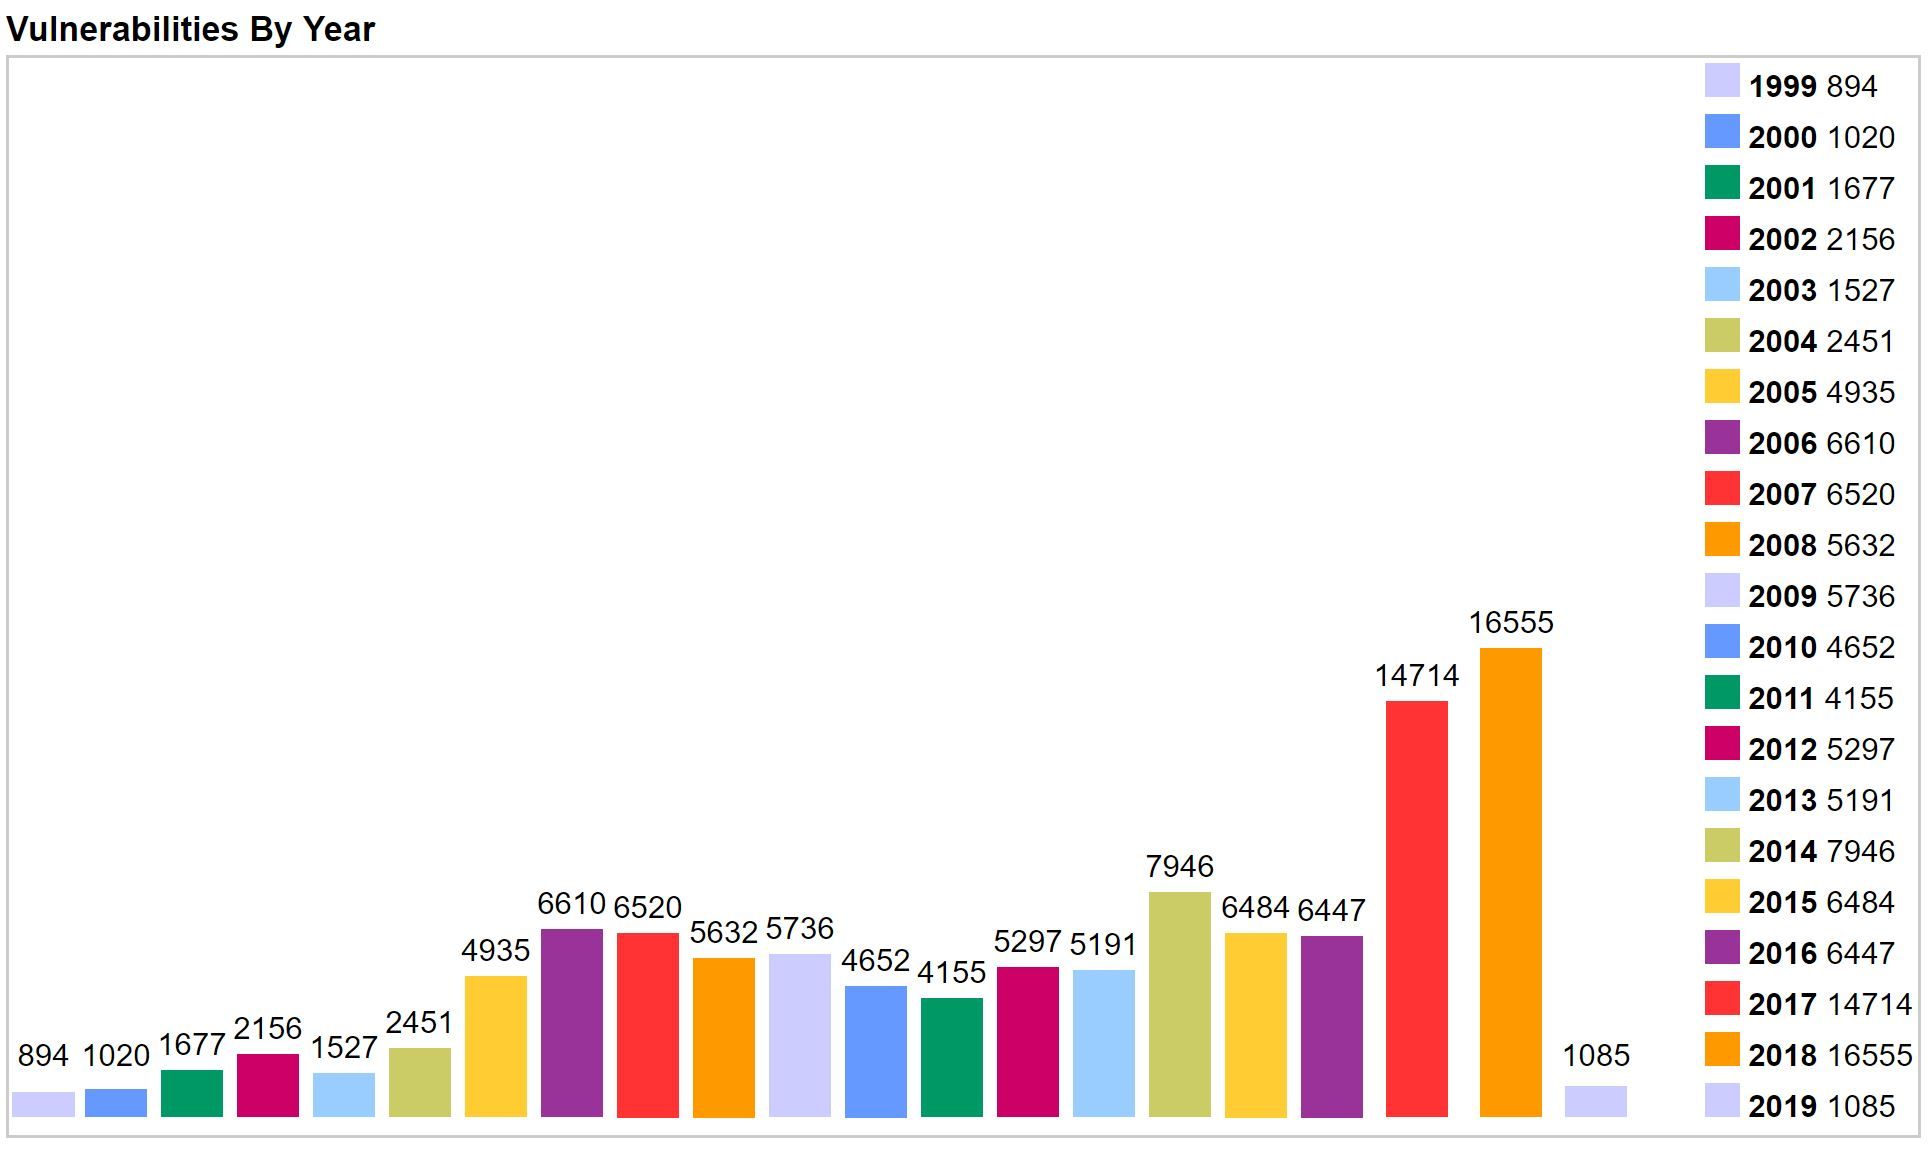
\includegraphics[width=1\textwidth]{Images/VulnByYear}
    \caption[Gefundene Schwachstellen pro Jahr laut CVE]{Gefundene Schwachstellen pro Jahr laut CVE \cite{cve}}
  \end{figure}

\chapter{Grundlagen}
  \section{Web Application Security}
    \subsection{Bedrohungen}
    TODO
      \subsubsection{OWASP Top 10}

    \subsection{Sicherheitsmaßnahmen}
    TODO

    \subsubsection{Web Application Firewalls (WAF)}
    TODO

    \subsubsection{Penetrationtesting}
    TODO

    \paragraph{Black-Box Testing}
    Beim Black-Box Testing befindet sich der Tester in der Rolle eines typischen Hackers von
    außen, der kein Wissen über die innere Arbeitsweise der Anwendung hat, weder Architektur noch
    Quellcode sind bekannt. Der Angreifer muss mit manuellen Methoden sowie speziellen Tools des Penetrationstestings vertraut sein, um Schwachstellen zu lokalisieren und auszunutzen. Für die dynamische Analyse des anzugreifenden Netzwerks benötigt er Scanning Tools, die in der vorliegenden Arbeit evaluiert werden.

    \paragraph{Grey-Box Testing}
    Während der Black-Box-Tester ein System aus der Sicht eines Außenseiters untersucht, hat ein    Grey-Box Tester bereits Zugriff auf das System auf Benutzerebene, möglicherwei- se sogar mit    erhöhten Berechtigungen eines Administrators. In der Regel liegt eine Dokumentation über Design und Architektur des Netzwerks vor, die internen Komponenten sind bekannt. Dies hat den Vorteil, dass die Sicherheit des Netzwerks gezielter und effizienter beurteilt werden kann, der Tester kann sich sofort auf die Systeme konzentrieren, die am wichtigsten sind oder ein besonders hohes Risiko haben. Zudem kann durch das interne Benutzerkonto ein Angriff innerhalb des abgesicherten Systems mit umfassendem Zugriff auf das Netzwerk simuliert werden.

    \paragraph{White-Box Testing}
    TODO
    \paragraph{Rechtliche Aspekte}
      \subparagraph{Hacker/Cracker vs. Pentester}
      TODO

  \section{Security Tools}
    \subsection{Mapping Tools}
    TODO
    \subsection{Scanning Tools}
    TODO
    \subsection{Exploitation Tools}
    TODO

\chapter{Methodik}
  \section{Testaufbau}
  Der Ablauf des Testens war für jeden WVS identisch.
  Zunächst wurden die verwundbare Web-Applikation gescannt und ein entsprechender Bericht generiert, anhand dessen die gefundenen Schwachstellen analysiert werden konnten. Dabei entstand ein subjektiver Eindruck der Handhabung und Bedienbarkeit, der zusammen mit dem Konfigurationsaufwand in die Evaluation einfließt. Um die True und False Positives zu identifizieren war es notwendig, die gefundenen Schwachstellen anhand von Dokumentationen der Websites oder manuell zu validieren und die Ergenisse zu vergleichen.

  Für die Tests wurde folgendes System verwendet:
  \\Intel Core i7-8700K CPU mit 32 GB RAM
  \\Microsoft Windows 10 pro, Version 1809 (64 bit)
  \\Als Virtuelle Maschinen innerhalb von VirtualBox: Kali Linux 18.4 und Parrot OS 4.5.1, jeweils ausgestattet mit 2 Kernen und 8 GB RAM

\section{Web Vulnerability Scanner (WVS)}
  \subsection{Auswahlkriterien}
  OWASP listet 50 verschiedene Tools zum Scannen von Web-Applications auf
  \cite{OWASPtools}. Die Auswahl wurde auf WVS mit folgenden Eigenschaften eingegrenzt:
  \begin{itemize}
    \item 1. Free und Open Source WVS.
    \item 2. Kommerzielle WVS, die eine voll funktionsfähige Testversion anbieten.
    \item 3. WVS, deren aktuelles Release nicht älter als 2 Jahre ist oder innerhalb der letzten 2 Jahre modifiziert wurde.
    \item 4. WVS, die in der Lage sind, umfassende Scans auszuführen, um möglichst viele verschiedene Schwachstellenarten aufzuspüren.
  \end{itemize}
  Bei den bekanntesten Anbietern kommerzieller WVS wurde jeweils eine Testversion angefragt, um ein realistisches Abbild der aktuell meistgenutzten Tools zu erhalten und um die Ergebnisse der kostenlosen denen der kommerziellen Scanner gegenüber zu stellen. Es handelt sich um folgende Firmen:
  \\Acunetix, Beyond Security (WSSA), Beyond Trust (Retina), Netsparker, N-Stalker, Portswigger (BurpSuite Pro), Rapid 7 (Nexpose) und Tenable (Nessus).

  Von den angefragten Firmen stellten Acunetix, Netsparker, N-Stalker, Portswigger und Tenable jeweils eine Testversion zur Verfügung.

  \subsection{Ausgewählte WVS}
    \subsubsection{Free und Open Source WVS}
      \begin{table}[H]
        \centering
          \begin{tabular}{|l|l|c|c|}
            \hline
            \textbf{WVS}              & \textbf{Entwickler}  & \textbf{Version}     & \textbf{Verwendete Plattform}  \\
            \hline
            \textbf{Arachni}          & Tasos Laskos         & 0.5.12 (WebUI)       & Windows                       \\
            \hline
            \textbf{Nikto}            & cirt.net             & 2.1.6                & Kali                          \\
            \hline
            \textbf{OpenVAS}          & Greenbone            & 7.0.3                & Parrot                        \\
            \hline
            \textbf{Wapiti}           & devloop              & 3.0.1                & Kali                          \\
            \hline
            \textbf{Zed Attack Proxy} & OWASP                & 2.7.0                & Parrot                        \\
            \hline
          \end{tabular}
        \caption[Ausgewählte Free und Open Source WVS]{Ausgewählte Free und Open Source WVS}
      \end{table}

    \subsubsection{Kommerzielle WVS}
      \begin{table}[H]
        \centering
          \begin{tabular}{|p{4cm}|l|c|c|}
            \hline
            \textbf{WVS}            & \textbf{Anbieter} & \textbf{Version} & \textbf{Verwendete Plattform}  \\
            \hline
            \textbf{Acunetix}       & Acunetix          & 12.0.190206130   & Kali                          \\
            \hline
            \textbf{Burp Suite Pro} & Portswigger       & 2.0.15           & Windows                       \\
            \hline
            \textbf{Nessus}         & Tenable           & 8.2.2            & Windows                       \\
            \hline
            \textbf{Netsparker}     & Netsparker        & 5.2.0.22027      & Windows                       \\
            \hline
          \end{tabular}
        \caption[Ausgewählte Kommerzielle WVS]{Ausgewählte Kommerzielle WVS}
      \end{table}

  \subsection{Nicht ausgewählte WVS}
    Nachfoldend werden alle WVS aufgelistet, die als Kandidaten in Erwägung gezogen wurden, bei näherer Betrachtung jedoch nicht die erforderlichen Voraussetzungen erfüllten, um in die Evaluation aufgenommen zu werden.
    \subsubsection{Free und Open Source WVS}
    \begin{itemize}
      \item GoLismero \cite{GoLismero}: GoLismero ist ein in Python geschriebenes Framework, das verschiedene Penetrationtesting-Tools in sich vereint. Theoretisch sollten bei einem Angriff alle Tools angewendet und die jeweiligen Ergebnisse in einem einzigen Report gebündelt werden. In der Praxis hängte sich das Programm jedoch jedes Mal nach einer Weile auf, sowohl unter Kali-Linux und Parrot OS, als auch unter Windows. Es werden zwar Teilergebnisse auf dem Bildschirm angezeigt, dies reicht aber nicht aus, um in die Evaluation aufgenommen zu werden.
      \item Grabber \cite{Grabber}: Das von Romain Gaucher entwickelte Programm ist zwar noch Bestandteil von Kali-Linux, ist aber schon über 12 Jahre alt (Latest Release 2006).
      \item Grendel-Scan \cite{Grendel}: Seit 2013 gibt es auf dem SourceForge-Repository von David Byrne keine Veränderung.
      \item Iron Wasp \cite{Iron}: Die aktuelle Verison des Windows-Programms von Lavakumar Kuppan ist ein Beta-Release aus dem Jahr 2015.
      \item Ratproxy \cite{Ratproxy}: Die Entwicklung wurde 2009 von Google eingestellt.
      \item Skipfish \cite{Skipfish}: Ein weiteres Projekt von Google, das 2012 eingestellt wurde.
      \item SQLmap \cite{SQLmap}: SQLmap ist ein beliebtes Tool zum Auffinden von SQLi Schwachstellen, ist aber darauf beschränkt.
      \item Vega \cite{Vega}: Das aktuelle Release ist aus dem Jahr 2014, seit diesem Jahr wird in regelmäßigen Abständen angekündigt, ein Feature zum Exportieren der Ergebnisse hinzuzufügen, aber die Firma Subgraph scheint das Projekt nicht weiter zu verfolgen.
      \item Watobo \cite{Watobo}: Die letzte Änderung des OpenSource Scanners stammt aus dem Jahr 2015.
      \item Webscarab \cite{Webscarab}: Der Vorgänger von OWASPs Zed Attack Proxy ist veraltet (Latest Release 2011), OWASP empfiehlt, auf ZAP umzusteigen.
      \item Wfuzz \cite{Wfuzz}: Der in Python geschriebene Scanner verwendet die Bibliothek Pycurl für HTTP-Requests, diese unterstützt keine SSL/TLS Verschlüsselung.
      \item W3af \cite{W3af}: W3af wird zwar noch sporadisch mit Bibliotheks-Aktualisierungen gepflegt, das aktuelle Release ist jedoch aus dem Jahr 2014 und es ist weder auf Kali-Linux noch auf Parrot OS gelungen, alle für den Programmstart benötigten Dependencies zu installieren. Das bei der Installation generierte Script versucht, teils veraltete Module zu installieren, manuelles Nachinstallieren der aktuellen Versionen brachte keinen Erfolg.
      \begin{figure}[H]
        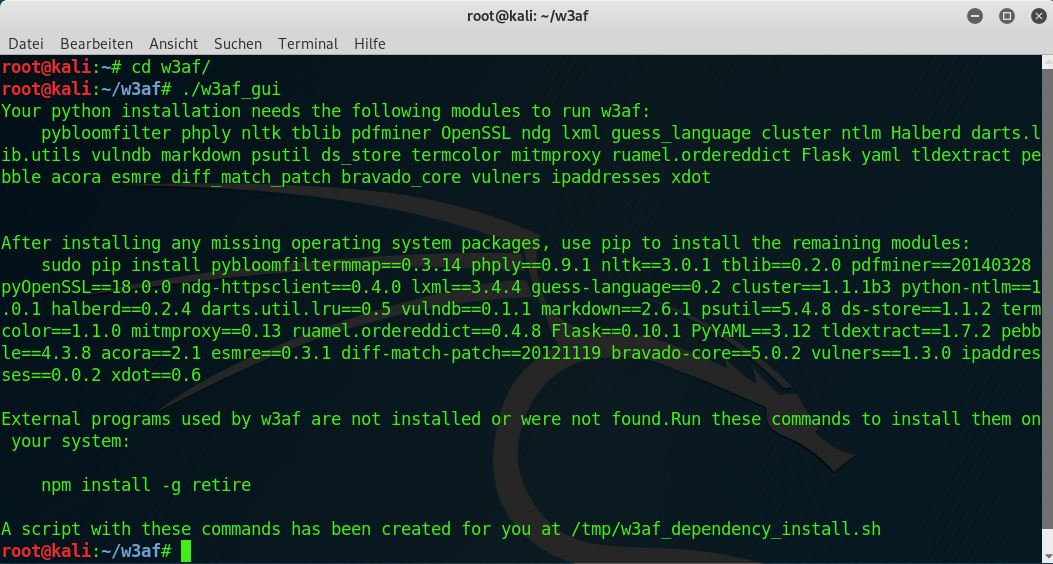
\includegraphics[width=1\textwidth]{Images/w3af}
        \caption[W3af: Fehlende Module]{W3af: Fehlende Module}
      \end{figure}
      \item Wikto \cite{Wikto}: Wikto ist eine Windows-Portierung von Nikto und bedarf daher keiner eigenen Evaluation.
      \item Xenotix \cite{Xenotix}: Xenotix wurde von OWASP für das Auffinden von Cross-Site-Scripting Schwachstellen entwickelt und ist darauf begrenzt.
    \end{itemize}
    \subsubsection{Kommerzielle WVS}
      \begin{itemize}
        \item N-Stalker \cite{Stalker}: Die angebotene ``7-Day Evaluation Licence'' erlaubt nur das Scannen einer einzigen, vorher festgelegten URL und ist daher für den geplanten Testaufbau nicht geeignet.
      \end{itemize}

\section{Verwundbare Web-Applikationen}
  Bei der Auswahl der Web-Applikationen musste darauf geachtet werden, dass sie für WVS geeignet sind. Auf ursprünglich in die Auswahl aufgenommene Applikationen wie WebGoat, JuiceShop (beide von OWASP) oder Damn Vulnerable Web Application (Bestandteil von Metasploitable) wurde am Ende verzichtet, da hier beim Scannen keine hinreichenden Ergebnisse hervorgebracht wurden. Diese Anwendungen  sind zwar sehr gut dokumentiert, aber hauptsächlich für das Erlernen von manuellen Angriffen entwickelt worden.
  %Um den Arbeitsaufwand bei der Validierung der Scan-Ergebnisse in einem angemessenen Rahmen zu halten, wurde nach der Testphase die Evaluation auf die Ergebnisse von fünf Web-Applikationen beschränkt. Hier wurden diejenigen bevorzugt, für die eine Schwachstellen-Dokumentation existiert. Nicht berücksichtigt wurden demzufolge die Resultate der Seiten Aspnet Testsparker \cite{Aspnet} und Crack Me Bank \cite{CrackMeBank}.
  Nachfolgend werden die für die Auswertung genutzten Web-Applikationen kurz vorgestellt.
  \subsection{Altoro Mutual}
    Altoro Mutual ist eine in C\texttt{\#} geschriebene Online-Banking Web-Applikation, die von IBM entwickelt wurde, um WVS zu testen \cite{Altoro}. Eine große Hilfe bei der Validierung der gefundenen Schwachstellen ist ein von IBM zur Verfügung gestellter Report, der sämtliche Schwachstellen der Seite auflistet \cite{IBM}.
  \subsection{Webscantest}
    Diese Web-Applikation ist in PHP geschrieben und wurde von NTOSpider entwickelt, um WVS zu testen. Die Schwachstellen sind direkt auf der Seite dokumentiert \cite{Webscantest}.
  \subsection{Zero Bank}
    Eine weitere Online-Banking Web-Applikation, entwickelt von Hewlett-Packard/Micro Focus \cite{Zero}. Auch hier gibt es einen gut dokumentierten Report mit allen Schwachstellen \cite{ZeroReport}.
  \subsection{Bitcoin Web Site}  \cite{Aspnet}
  \subsection{Acuart}
    Eine Test-Seite von Acunetix, der einen Online-Shop für Kunstwerke simuliert, geschrieben in PHP \cite{Acuart}.
  \subsection{Crack Me Bank} \cite{CrackMeBank}
  \subsection{Security Tweets}
    Security Tweets ist eine von Twitter inspirierte Social Networks Applikation, die ebenfalls von Acunetix entwickelt wurde. Sie ist in HTML5 geschrieben \cite{Tweets}.
\chapter{Evaluation}
  \section{Gefundene Schwachstellen per Web Application}
  TODO
  \section{Gefundene Schwachstellen nach Schwachstellentyp}
  TODO
  \section{Bedienung, Geschwindigkeit und Konfigurationsaufwand}
   Für die Bewertung wurde eine Skala mit fünf Skalenwerten von -{}- bis ++ herangezogen:
   \begin{table}[H]
      \begin{tabular}{ll}
      -{}-         & \textbf{ungenügend}             \\
      -            & \textbf{unterdurchschnittlich}  \\
      o            & \textbf{durchschnittlich}       \\
      +            & \textbf{überdurchschnittlich}   \\
      ++           & \textbf{überragend}
      \end{tabular}
    \end{table}
    Das Gesamtergebnis setzt sich aus den Bewertungen für die Bedienung (20\%), der Geschwindigkeit (20\%) und dem Scanergebnis (60\%) zusammen.

    \subsection{Open Source}
      \begin{table}[H]
        \centering
        \begin{tabular}{|r|c|c|c|c|c|}
        \hline
        \textbf{Open Source WVS}            & \textbf{Arachni} & \textbf{Nikto} & \textbf{OpenVAS} & \textbf{Wapiti} & \textbf{Zed Attack Proxy}  \\
        \hline
        \textbf{Bedienung (20\%)}       & \textbf{+}       & \textbf{o}     & \textbf{-}       & \textbf{o}      & \textbf{+}                 \\
        \hline
        \textbf{Geschwindigkeit (20\%)} & \textbf{+}       & \textbf{++}    & \textbf{o}       & \textbf{++}     & \textbf{-{}-}                \\
        \hline
        \textbf{Scanergebnis (60\%)}    &                  &                &                  &                 &                            \\
        \hline
        \textbf{Gesamt}                 &                  &                &                  &                 &                            \\
        \hline
        \end{tabular}
        \caption[Bewertung der Open Source WVS]{Bewertung der Open Source WVS}
      \end{table}

        \begin{itemize}
          \item Arachni \cite{Arachni}:\\
            Arachni gibt es als reine Terminal-Anwendung oder als Ruby on Rails Framework mit Web-Interface. Die Web-Oberfläche ist übersichtlich und verständlich aufgebaut, der User findet sich schnell zurecht und kann sofort mit dem Scannen einer Seite beginnen, die Scangeschwindigkeit ist überdurchschnittlich. Als Hilfestellung gibt es ein umfangreiches Wiki mit Erklärungen und Screenshots.
            \begin{figure}[H]
              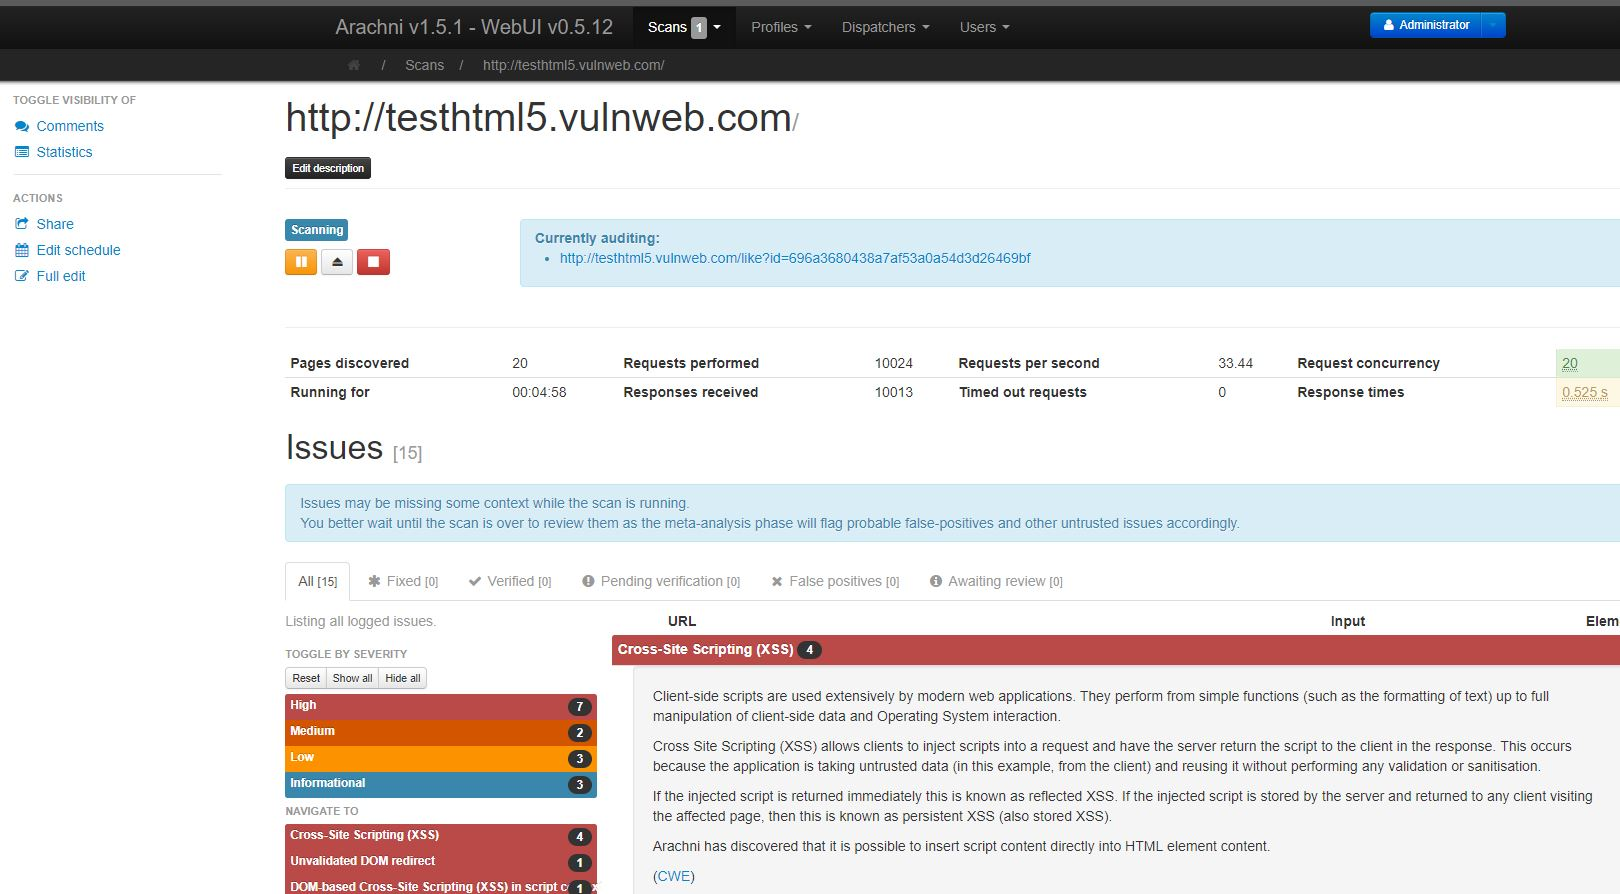
\includegraphics[width=1\textwidth]{Images/Arachni}
              \caption[Arachni WebUI 0.5.12]{Arachni WebUI 0.5.12}
            \end{figure}
          \item Nikto \cite{Nikto}:\\
            Nikto ist ein gut dokumentiertes Terminal-Programm, nach kurzer Einarbeitung hat ein ungeübter User die benötigten Befehle und Optionen gefunden, um einen Scan zu starten.
            Auffällig ist die im Vergleich zu allen anderen WVS ungewöhnlich hohe Scan-Geschwindigkeit, die sich im Minutenbereich einordnet.
            Der generierte Report listet alle gefundenen Schwachstellen detailliert auf, unterscheidet diese jedoch im Gegensatz zu den meisten anderen WVS nicht zwischen High, Medium, Low und Informational.
          \item OpenVAS \cite{OpenVAS}:\\
            OpenVAS ist aus der Software Nessus hervorgegangen, als diese im Jahr 2005 von Open Soucre zu einer kommerziellen Lizenz wechselte, und wird seitdem auf Basis der letzten freien Nessus-Version 2.2 von Greenbone Networks weiterentwickelt. Der Scanner ist eingebettet in den Greenbone Security Assistant, der über ein Web-Interface bedient wird. Die Oberfläche ist nicht selbsterklärend, es bedarf etwas an Recherche, bis sich dem User der logische Aufbau des Programms erschließt. Hier ist das ``Tech Doc-Portal'' von Greenbone sehr hilfreich. Zuerst muss unter Configuration/Targets ein Ziel definiert werden, dann kann der User für dieses Ziel unter dem Punkt ``Scans'' einen Task erstellen und diesen entweder sofort oder per Schedule starten.
            Die umständliche Handhabung hat den Vorteil, dass sich leicht mehrere Tasks automatisieren lassen.
            \begin{figure} [H]
              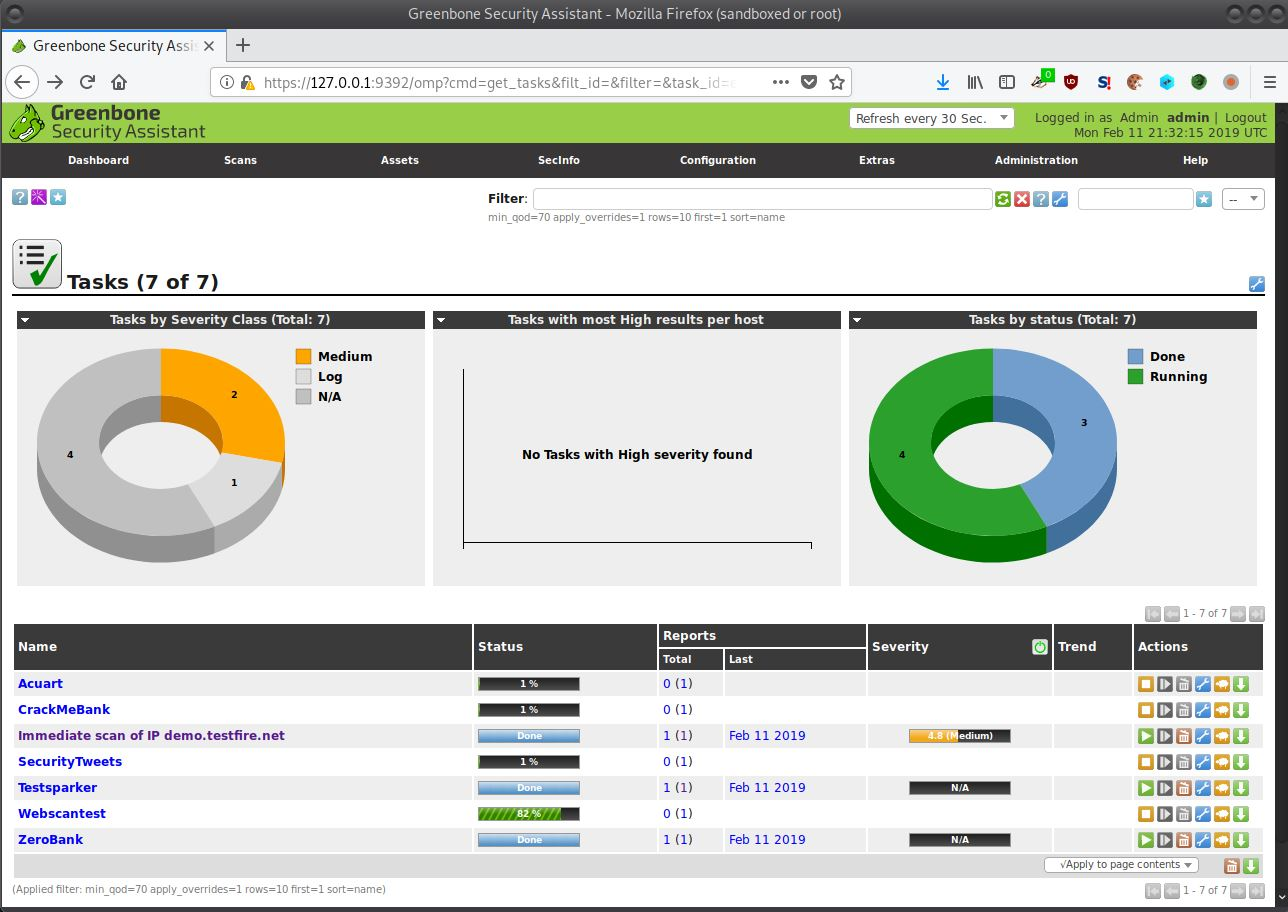
\includegraphics[width=1\textwidth]{Images/OpenVAS}
              \caption[OpenVAS im Greenbone Security Assistant]{OpenVAS im Greenbone Security Assistant}
            \end{figure}
          \item Wapiti \cite{Wapiti}:\\
            In der Handhabung und im Reporting ähnelt Wapiti dem anderen reinen Terminal-Programm Nikto. Die auswählbaren Optionen sind ähnlich, und die gefundenen Schwachstellen werden auch hier nicht in Kategorien eingeteilt. Die Dokumentation fällt etwas spartanischer aus, ist aber ausreichend, um sich schnell zurecht zu finden. Wapiti scannt nicht so schnell wie Nikto, reiht sich aber im oberen Mittelfeld ein.

          \item Zed Attack Proxy \cite{ZAP}:\\
            Der von OWASP entwickelte Scanner hat eine übersichtliche Benutzeroberfläche und lässt sich intuitiv bedienen. Auf der Startseite lässt sich direkt die anzugreifende URL eingeben und ohne weitere Konfiguration angreifen. Es gibt umfangreiche Hilfestellung in Form eines Handbuchs und einem Online-Wiki, zudem gibt es mit der OWASP ZAP User Group ein gut frequentiertes Benutzerforum, auf dem ein reger Austausch zwischen den Benutzern stattfindet.
            Auffällig sind die langen Scan-Zeiten von mehreren Stunden, die sich jedoch nicht in einer höheren Anzahl an gefundenen Schwachstellen widerspiegeln.
          \begin{figure}[H]
            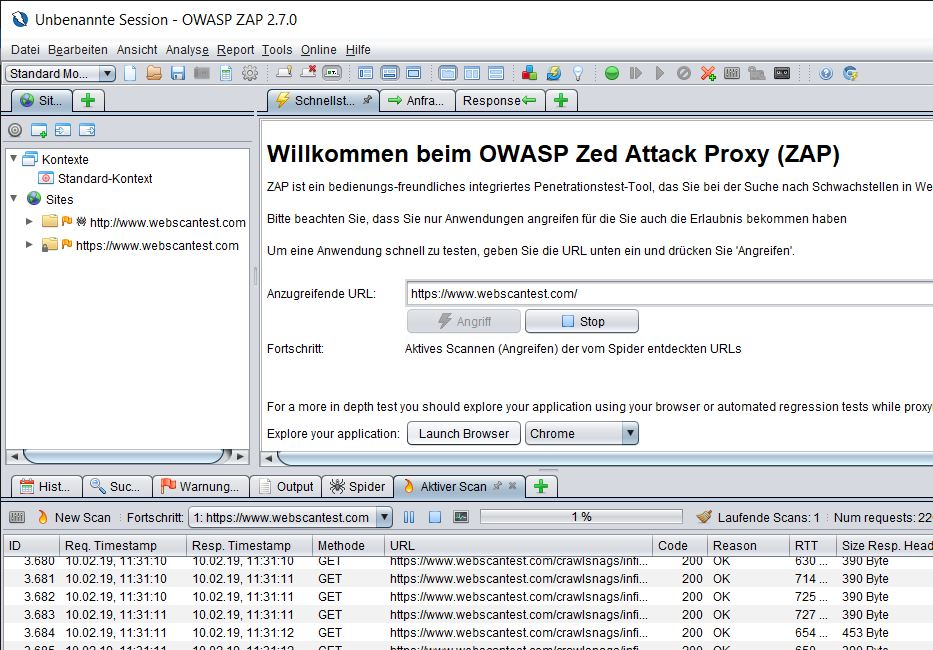
\includegraphics[width=1\textwidth]{Images/ZAP}
            \caption[Grafische Benutzeroberfläche von ZAP]{Grafische Benutzeroberfläche von ZAP}
          \end{figure}
        \end{itemize}

    \subsection{Kommerziell}
    \begin{table}[H]
      \centering
      \begin{tabular}{|r|c|c|c|c|}
      \hline
      \textbf{Kommerzielle WVS}       & \textbf{Acunetix} & \textbf{Burp Suite Pro} & \textbf{Nessus} & \textbf{Netsparker}  \\
      \hline
      \textbf{Bedienung (20\%)}       & \textbf{-}        & \textbf{+}              & \textbf{+}      & \textbf{o}           \\
      \hline
      \textbf{Geschwindigkeit (20\%)} & \textbf{++}       & \textbf{o}              & \textbf{o}      & \textbf{-}           \\
      \hline
      \textbf{Scanergebnis (60\%)}    &                   &                         &                 &                      \\
      \hline
      \textbf{Gesamt}                 &                   &                         &                 &                      \\
      \hline
      \end{tabular}
      \caption[Bewertung der kommerziellen WVS]{Bewertung der kommerziellen WVS}
    \end{table}
      \begin{itemize}
        \item Acunetix \cite{Acunetix}:\\
          Acunetix stellte eine 14-tägige Vollversion zur Verfügung. Die graphische Oberfläche ist sehr übersichtlich und lässt sich intuitiv bedienen. Online gibt es ein Support-Portal mit ausführlicher Dokumentation und Hilfestellung.
          Unter Windows brachte Acunetix das System mehrmals zum Absturz (BSOD), so dass auf die Linux-Version ausgewichen wurde. Hier lief das Programm stabil und scannte von den kommerziellen WVS am schnellsten, von allen WVS muss sich Acunetix hier nur von Wapiti und Nikto geschlagen geben.
          \begin{figure}[H]
            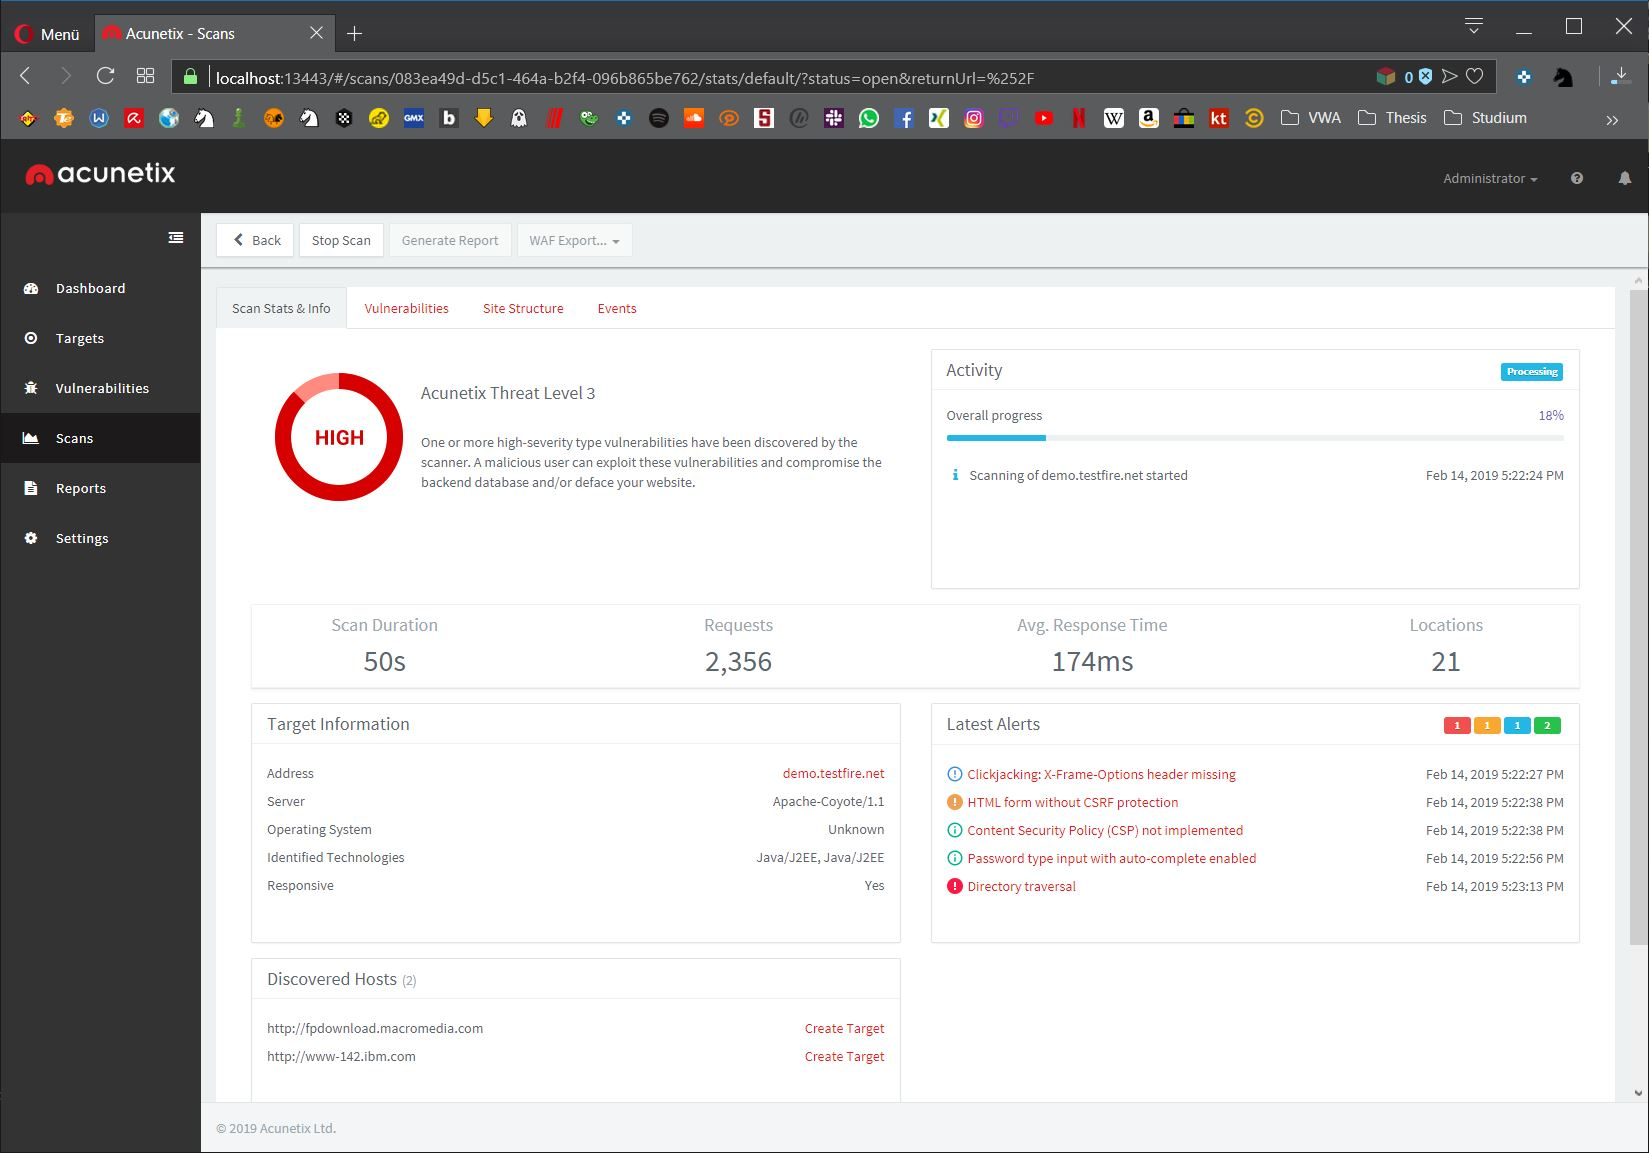
\includegraphics[width=1\textwidth]{Images/Acunetix}
            \caption[Weboberfläche von Acunetix]{Weboberfläche von Acunetix}
          \end{figure}
        \item BurpSuite Pro \cite{Burp}:\\
          Die Firma Portswigger stellte auf Anfrage eine 30-tägige unbeschränkte Testversion zur Verfügung.
          BurpSuite Pro enthält eine umfangreiche Dokumentation mit zahlreichen Hilfestellungen für verschiedene Anwendungsszenarien.  Das Dashboard ist sehr übersichtlich und intuitiv zu bedienen: mit Hilfe des Buttons ``New Scan'' lässt sich direkt ohne größeren Konfigurationsaufwand eine Website erfolgreich und in durchschnittlicher Geschwindigkeit scannen.
          \begin{figure}[H]
            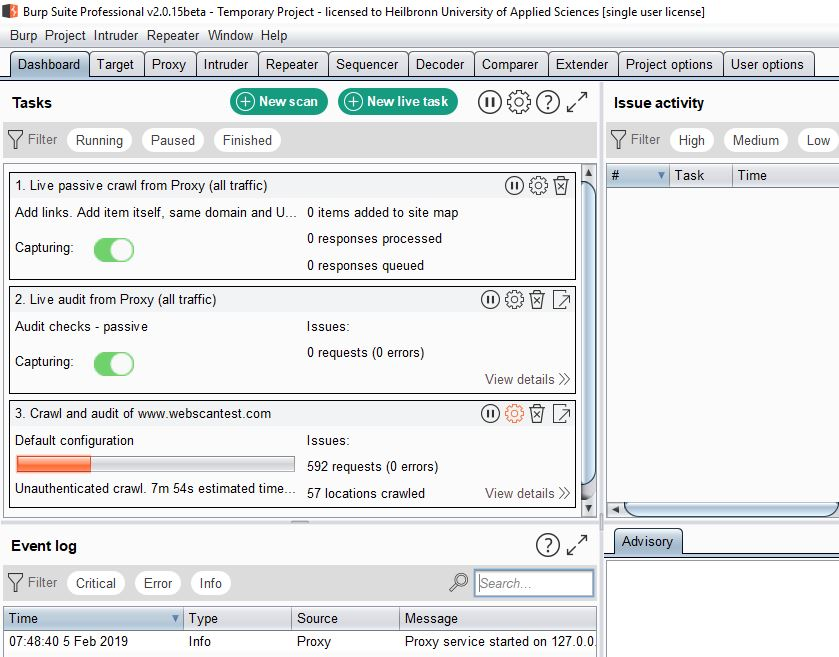
\includegraphics[width=1\textwidth]{Images/BurpSuitePro}
            \caption[Dashboard von BurpSuite Pro]{Dashboard von BurpSuite Pro}
          \end{figure}
        \item Nessus \cite{Nessus}:\\
          Die Firma Tenable bietet zwei Testversionen an: Nessus Home für das Testen des heimischen Netzwerks, gültig für ein Jahr sowie eine unbeschränkte Version von Nessus Pro, gültig für sieben Tage.
          Nessus präsentiert sich auf einer übersichtlich gestalteten Web-Schnittstelle und ist selbsterklärend bedienbar. Einen Hilfe-Button sucht man vergeblich, die umfangreiche Dokumentation mit Anleitungen findet man online durch recherchieren. Die Scangeschwindigkeit ist durchschnittlich.
          \begin{figure}[H]
            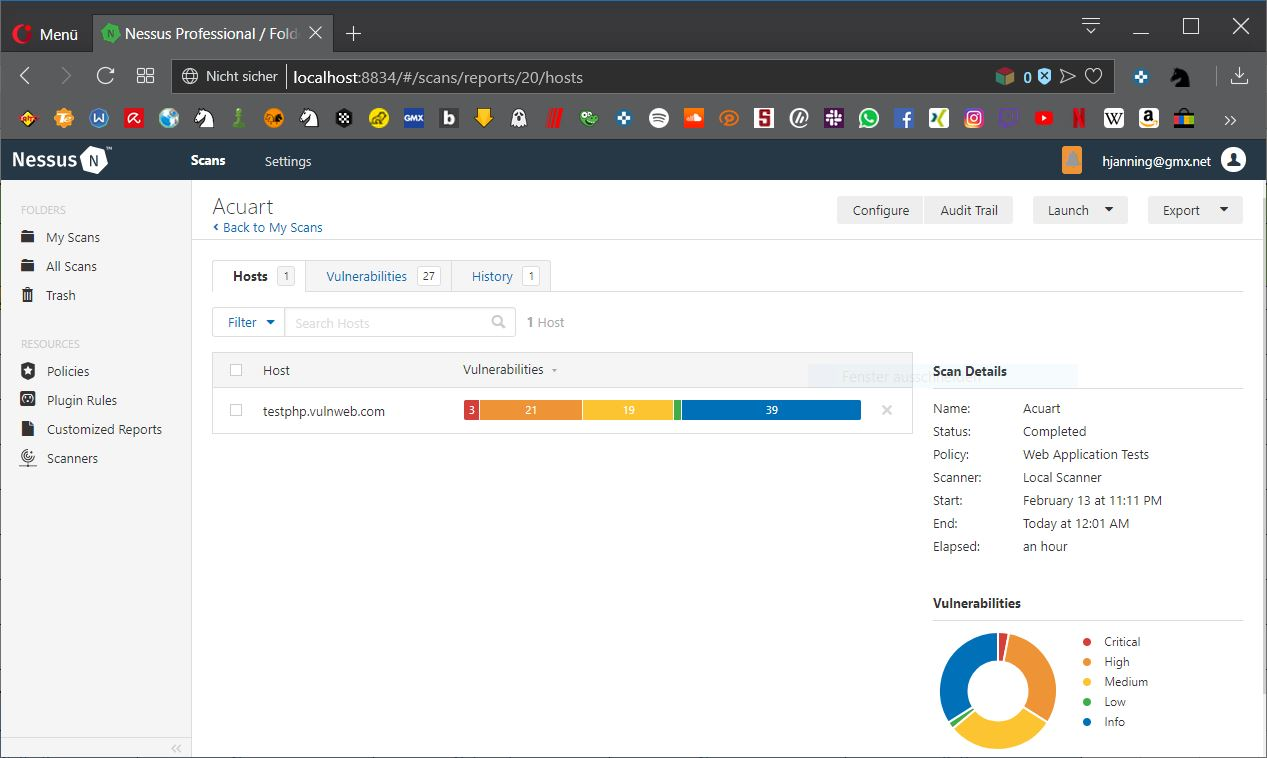
\includegraphics[width=1\textwidth]{Images/Nessus}
            \caption[Grafische Benutzeroberfläche von Nessus]{Grafische Benutzeroberfläche von Nessus}
          \end{figure}
        \item Netsparker \cite{Netsparker}:\\
          Netsparker stellte nach Rücksprache eine 14-tägige Testversion zur Verfügung, die auf 8 zu scannende Web-Applikationen begrenzt ist. Die grafische Benutzeroberfläche ist etwas unruhig und überladen, der User kann aber direkt über den Button ``New'' eine Web-Seite scannen. Die Scangeschwindigkeit ist im unteren Mittelfeld angesiedelt.
          \begin{figure}[H]
            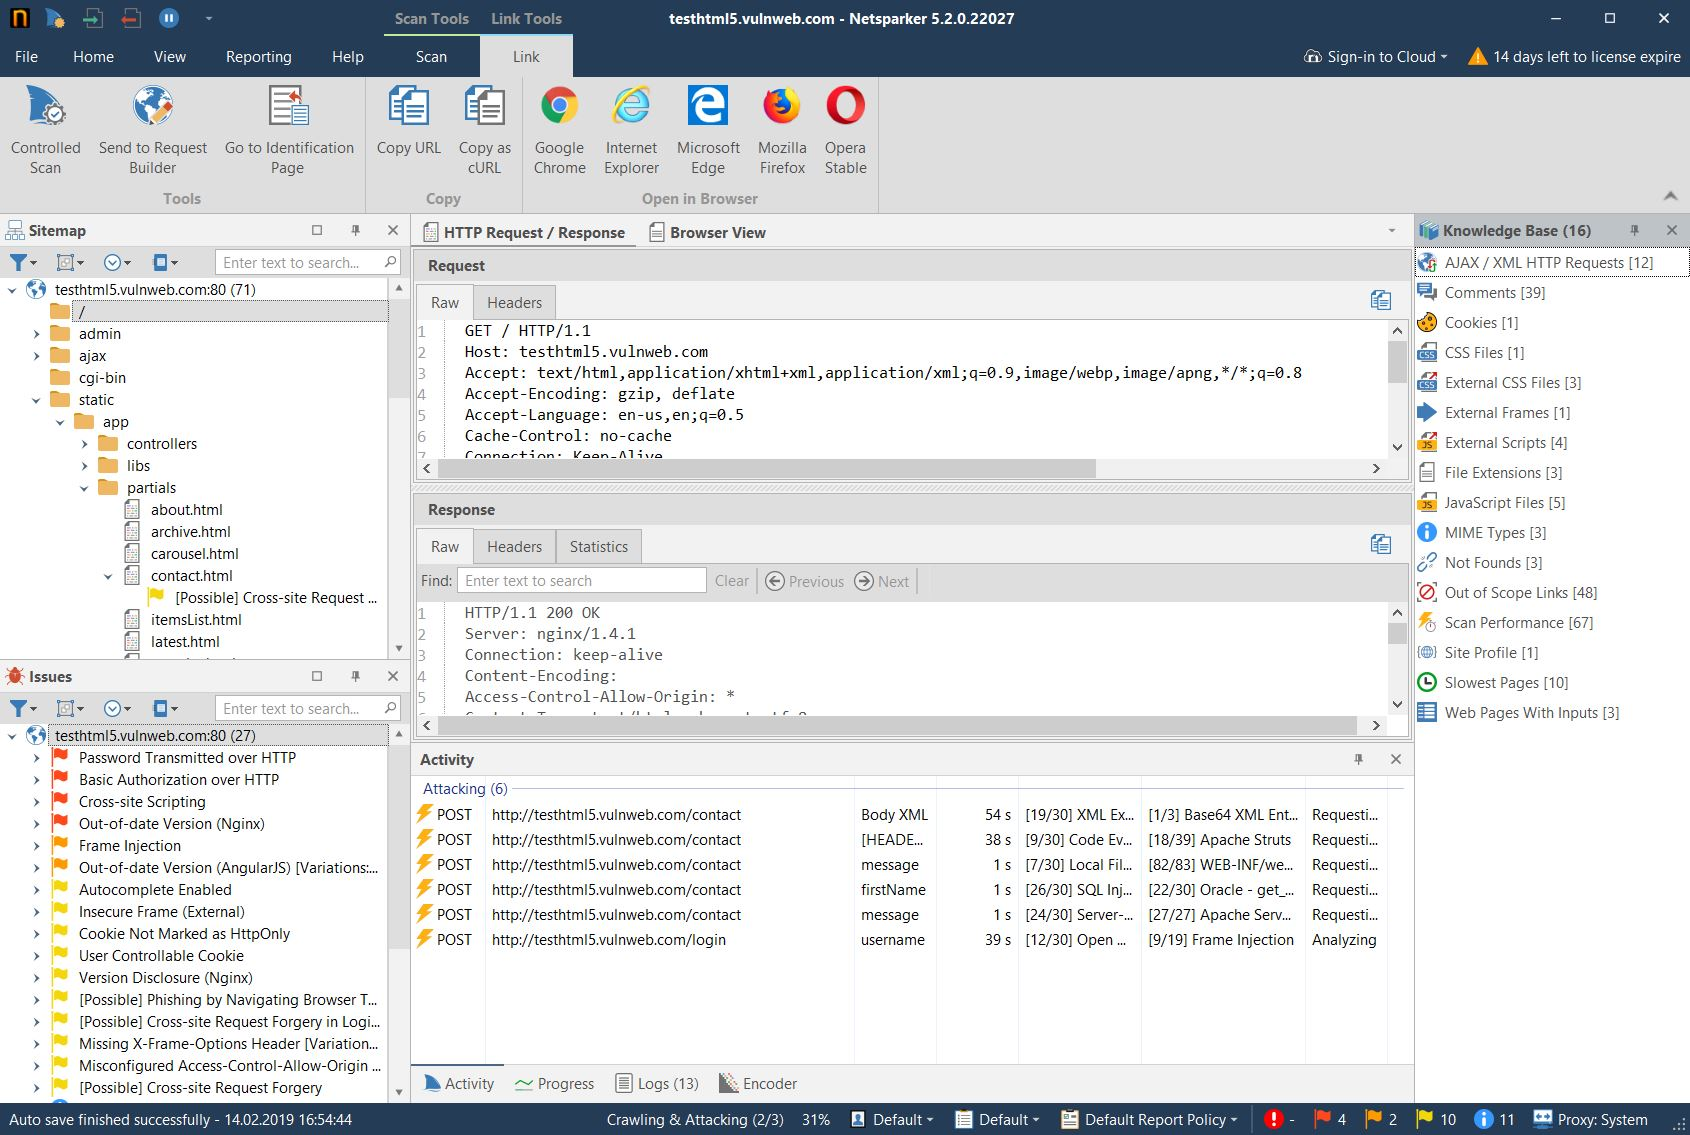
\includegraphics[width=1\textwidth]{Images/Netsparker}
            \caption[Grafische Benutzeroberfläche von Netsparker]{Grafische Benutzeroberfläche von Netsparker}
          \end{figure}
     \end{itemize}

\chapter{Diskussion}
  \section{Open Source WVS}
    \begin{itemize}
      \item

    \end{itemize}
  \section{Kommerzielle WVS}
  TODO
  \section{Open Source vs. kommerziell}
  TODO
  \section{Empfehlung}


\chapter{Fazit und Ausblick}
TODO
  \section{OWASP Benchmark}
  TODO


\backmatter


%%%%%%%%%%%%%%%%%%%
%% create listings list
%%%%%%%%%%%%%%%%%%%
%\lstlistoflistings
%\addcontentsline{toc}{chapter}{Listings}

\cleardoublepage
\phantomsection
\addcontentsline{toc}{chapter}{Quellenverzeichnis}
\printbibliography[title=Quellenverzeichnis]

\appendix
  \chapter*{Anhang}
  \addtocontents{toc}{\protect{\vspace{3ex}}}
  \addcontentsline{toc}{chapter}{Anhang}

  \section{Verwendete Abk"urzungen}
  \dots{}

  \section{OWASP: The Open Web Application Security Project}
  Das ``Open Web Application Security Project'' (OWASP) ist eine unabhängige, weltweite Community mit dem Ziel, die Bedeutung der Sicherheit von Webanwendungen »sichtbar zu machen«, Fachwissen zur Entwicklung und den Betrieb sicherer Webanwendungen zu verbreiten und frei zur Verfügung zu stellen.
  OWASP ist mit keinem Technologieunternehmen verbunden, obwohl der Einsatz kommerzieller Sicherheitstechnologien unterstützt wird. Sämtliche OWASP-Instrumente, wie Dokumente, Videos, Slides, Podcasts etc. sind kollaborativ produziert worden und sind zudem kostenlos unter einer freien Lizenz verwendbar. Die OWASP Foundation ist eine Non-Profit-Organisation, die sich vier Grundwerten verschrieben hat \cite{OWASPabout}:
  \begin{itemize}
    \item Offenheit: Von den Finanzen bis zum Code ist alles radikal transparent.
    \item Innovation: OWASP fördert und unterstützt Innovationen und Experimente zur Lösung von Software-Sicherheitsherausforderungen.
    \item Globalität: Jeder auf der ganzen Welt kann sich an der OWASP-Community beteiligen.
    \item Integrität: OWASP ist eine ehrliche und aufrichtige, herstellerneutrale, globale Gemeinschaft.
  \end{itemize}
  Zudem gibt es einen Verhaltenskodex mit folgenden Prinzipien:
  \begin{itemize}
    \item Führe alle beruflichen Tätigkeiten und Pflichten in Übereinstimmung mit allen anwendbaren Gesetzen und den höchsten ethischen Grundsätzen aus.
    \item Fördere die Umsetzung von Normen, Verfahren und Kontrollen für die Anwendungssicherheit und deren Einhaltung.
    \item Bewahre eine angemessenene Vertraulichkeit gegenüber geschützter oder anderweitig sensibler Informationen, die im Rahmen einer beruflichen Tätigkeit auftreten.
    \item Übernimm die berufliche Verantwortung mit Sorgfalt und Ehrlichkeit.
    \item Kommuniziere offen und ehrlich.
    \item Vermeide Aktivitäten, die einen Interessenskonflikt hervorrufen oder anderweitig den Ruf des Arbeitgebers, den Informationssicherheitsberuf oder die Vereinigung beeinträchtigen könnten.
    \item Bewahre und verstärke unsere Objektivität und Unabhängigkeit.
    \item Weise unangemessenen Druck der von Seiten der Industrie oder anderen zurück.
    \item Verletze oder bestreite nicht absichtlich den Ruf von Kollegen, Kunden oder Arbeitgebern.
    \item Behandle jeden mit Respekt und Würde.
    \item Vermeide Beziehungen, die die Objektivität und Unabhängigkeit von OWASP  beeinträchtigen könnten.
  \end{itemize}
    \subsection{Die OWASP Top Ten}
    TODO
     \cite{OWASPtop10}

    \subsubsection{A1: Injection}
    Injection-Schwachstellen, wie beispielsweise SQL-, OS- oder LDAP-Injection, treten auf, wenn
    nicht vertrauenswürdige Daten von einem Interpreter als Teil eines Kommandos oder einer
    Abfrage verarbeitet werden. Ein Angreifer kann Eingabedaten dann so manipulieren, dass er nicht
    vorgesehene Kommandos ausführen oder unautorisiert auf Daten zugreifen kann.

    \subsubsection{A2: Fehler in der Authentifizierung}
    Anwendungsfunktionen, die im Zusammenhang mit Authentifizierung und Sessionmanagement
    stehen, werden häufig fehlerhaft implementiert. Dies erlaubt es Angreifern, Passwörter oder
    Session-Token zu kompromittieren oder die entsprechenden Schwachstellen so auszunutzen,
    dass sie die Identität anderer Benutzer vorübergehend oder dauerhaft annehmen können.

    \subsubsection{A3: Verlust der Vertraulichkeit sensibler Daten}
    Viele Anwendungen schützen sensible Daten, wie personenbezogene Informationen und Finanzoder
    Gesundheitsdaten, nicht ausreichend. Angreifer können diese Daten auslesen oder
    modifizieren und mit ihnen weitere Straftaten begehen (Kreditkartenbetrug, Identitätsdiebstahl
    etc.). Vertrauliche Daten können kompromittiert werden, wenn sie nicht durch Maßnahmen, wie
    Verschlüsselung gespeicherter Daten und verschlüsselte Datenübertragung, zusätzlich geschützt
    werden. Besondere Vorsicht ist beim Datenaustausch mit Browsern angeraten.

    \subsubsection{A4: XML External Entities}
    Viele veraltete oder schlecht konfigurierte XML Prozessoren berücksichtigen Referenzen auf
    externe Entitäten innerhalb von XML-Dokumenten. Dadurch können solche externen Entitäten
    dazu eingesetzt werden, um mittels URI Datei-Handlern interne Dateien oder File-Shares offenzulegen
    oder interne Port-Scans, Remote-Code-Executions oder Denial-of-Service Angriffe
    auszuführen.

    \subsubsection{A5: Fehler in der Zugriffskontrolle}
    Häufig werden die Zugriffsrechte für authentifizierte Nutzer nicht korrekt um- bzw. durchgesetzt.
    Angreifer können entsprechende Schwachstellen ausnutzen, um auf Funktionen oder Daten
    zuzugreifen, für die sie keine Zugriffsberechtigung haben. Dies kann Zugriffe auf Accounts
    anderer Nutzer sowie auf vertrauliche Daten oder aber die Manipulation von Nutzerdaten,
    Zugriffsrechten etc. zur Folge haben.

    \subsubsection{A6: Sicherheitsrelevante Fehlkonfiguration}
    Fehlkonfigurationen von Sicherheitseinstellungen sind das am häufigsten auftretende Problem.
    Ursachen sind unsichere Standardkonfigurationen, unvollständige oder ad-hoc durchgeführte
    Konfigurationen, ungeschützte Cloud-Speicher, fehlkonfigurierte HTTP-Header und Fehlerausgaben,
    die vertrauliche Daten enthalten. Betriebssysteme, Frameworks, Bibliotheken und Anwendungen
    müssen sicher konfiguriert werden und zeitnah Patches und Updates erhalten.

    \subsubsection{A7: Cross-Site-Scripting (XSS)}
    XSS tritt auf, wenn Anwendungen nicht vertrauenswürdige Daten entgegennehmen und ohne
    Validierung oder Umkodierung an einen Webbrowser senden. XSS tritt auch auf, wenn eine
    Anwendung HTML- oder JavaScript-Code auf Basis von Nutzereingaben erzeugt. XSS erlaubt es
    einem Angreifer, Scriptcode im Browser eines Opfers auszuführen und so Benutzersitzungen zu
    übernehmen, Seiteninhalte verändert anzuzeigen oder den Benutzer auf bösartige Seiten
    umzuleiten.

    \subsubsection{A8: Unsichere Deserialisierung}
    Unsichere, weil unzureichend geprüfte Deserialisierungen können zu Schwachstellen in der
    Remote-Code-Execution führen. Aber auch wenn das nicht der Fall ist, können
    Deserialisierungsfehler Angriffsmuster wie Replay-Angriffe, Injections und Erschleichung
    erweiterter Zugriffsrechte ermöglichen.

    \subsubsection{A9: Nutzung von Komponenten mit bekannten Schwachstellen}
    Komponenten wie Bibliotheken, Frameworks etc. werden mit den Berechtigungen der zugehörigen
    Anwendung ausgeführt. Wird eine verwundbare Komponente ausgenutzt, kann ein solcher
    Angriff von Datenverlusten bis hin zu einer Übernahme des Systems führen. Applikationen und
    APIs, die Komponenten mit bekannten Schwachstellen einsetzen, können Schutzmaßnahmen
    unterlaufen und so Angriffe mit schwerwiegenden Auswirkungen verursachen.

    \subsubsection{A10: Unzureichendes Logging und Monitoring}
    Unzureichendes Logging und Monitoring führt zusammen mit fehlender oder uneffektiver Reaktion auf Vorfälle zu andauernden oder wiederholten Angriffen. Auch können Angreifer dadurch in Netzwerken weiter vordringen und Daten entwenden, verändern oder zerstören. Viele Studien zeigen, dass die Zeit bis zur Aufdeckung eines Angriffs bei ca. 200 Tagen liegt sowie typischerweise durch Dritte entdeckt wird und nicht durch interne Überwachungs- und Kontrollmaßnahmen.


%%%%%%%%%%%%%%%%%%%
%% declaration on oath
%%%%%%%%%%%%%%%%%%%

\addchap{Eidesstattliche Erklärung}

Hiermit versichere ich, dass ich die vorgelegte Bachelorarbeit selbstständig verfasst und noch nicht anderweitig zu Prüfungszwecken vorgelegt habe. Alle benutzten Quellen und Hilfsmittel sind angegeben, wörtliche und sinngemäße Zitate wurden als solche gekennzeichnet.

\vspace{20pt}
\begin{flushright}
$\overline{~~~~~~~~~~~~~~~~~\mbox{\BaAuthor, am \today}~~~~~~~~~~~~~~~~~}$
\end{flushright}




\end{document}
